\documentclass{../../slides-style}

\slidetitle[Практика]{Многопоточное программирование}{21.09.2022}

\begin{document}

    \begin{frame}[plain]
        \titlepage
    \end{frame}

    \begin{frame}
        \frametitle{Deadlock}
        \begin{center}
            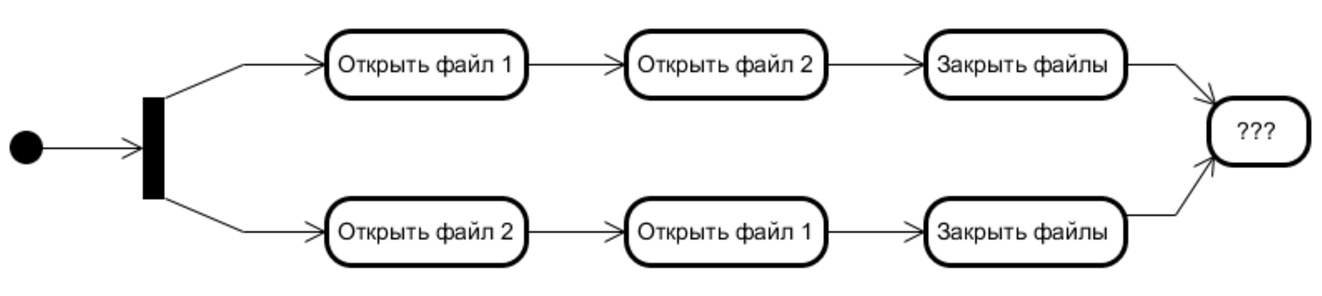
\includegraphics[width=0.9\textwidth]{deadlock.png}
        \end{center}
    \end{frame}
    
    \begin{frame}
        \frametitle{Условия взаимной блокировки}
        \begin{enumerate}
            \item имеется разделяемый ресурс, к которому потоки хотят получить доступ, но пользоваться им может только один поток
            \item таких ресурсов несколько, и поток, захватив один, хочет получить доступ к другим, которые в этот момент захвачены другими потоками
            \item нельзя отнять захваченный ресурс у потока
            \item потоки ждут друг друга <<по кругу>>
        \end{enumerate}
        Блокировка возможна, только если выполнены сразу все эти условия.
    \end{frame}

    \begin{frame}
        \frametitle{Задача, ``Обедающие философы''}
        \begin{columns}
            \begin{column}{0.5\textwidth}
                \begin{itemize}
                    \item Есть N тарелок спагетти, N вилок и N философов
                    \item Философ может думать и есть
                    \item Чтобы есть, философу нужны две вилки
                    \item Пример --- транзакция, переводящая деньги со счёта на счёт
                \end{itemize}
            \end{column}
            \begin{column}{0.5\textwidth}
                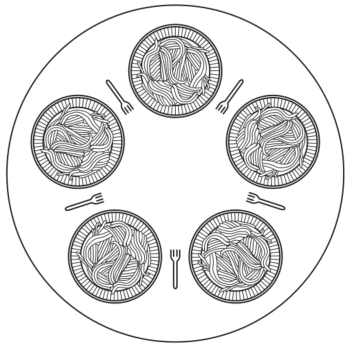
\includegraphics[width=0.9\textwidth]{diningPhilosophers.png}
                \attribution{A. Tanenbaum, Modern Operating Systems}
            \end{column}
        \end{columns}
    \end{frame}

    \begin{frame}
        \frametitle{Что надо сделать}
        \begin{itemize}
            \item Смоделировать ситуацию обедающих философов
            \begin{itemize}
                \item Придумать красивую объектно-ориентированную модель
                \item Каждый философ живёт независимо, поэтому в отдельном потоке
                \item Вилке не нужен свой отдельный класс
            \end{itemize}
            \item Выводить на экран состояния философов
            \item Считаем, что философы думают и едят случайное, но небольшое количество времени
            \item Реализация должна гарантировать отсутствие взаимоблокировок
            \item Нужно уметь корректно останавливать процесс и распускать философов по домам
        \end{itemize}
    \end{frame}

\end{document}
